\documentclass{article}
\usepackage{multicol}
\usepackage[utf8]{inputenc}
\usepackage{float}
\usepackage{graphicx}
\usepackage{hyperref}
\hypersetup{
    colorlinks=true,
    urlcolor=blue,
    }
    
\usepackage{geometry}
\geometry{
    a4paper,
    total={170mm,257mm},
    left=30mm,
    right=30mm,
    top=20mm,
    }

\usepackage{forest}
\definecolor{folderbg}{RGB}{124,166,198}
\definecolor{folderborder}{RGB}{110,144,169}
\def\Size{4pt}
\tikzset{
  folder/.pic={
    \filldraw[draw=folderborder,top color=folderbg!50,bottom color=folderbg]
      (-1.05*\Size,0.2\Size+5pt) rectangle ++(.75*\Size,-0.2\Size-5pt);  
    \filldraw[draw=folderborder,top color=folderbg!50,bottom color=folderbg]
      (-1.15*\Size,-\Size) rectangle (1.15*\Size,\Size);
  }
}

% ------------------------------- FRONT MATTER ------------------------------- %

\title{\textbf{GreenBook}\\~\\
    Third assignment\\
    \small Software Development Process course\\
        University of Milano - Bicocca\\
        A.A. 2021/22\\~\\
        \href{https://gitlab.com/massimino96/2021_assignment3_greenbook/}{Repository Link}}
\author{Authors:\\
    830260 - Binda Paolo - \href{mailto:p.binda@campus.unimib.it}{p.binda@campus.unimib.it}\\
    831075 - D'Apa Massimo - \href{mailto:m.dapa@campus.unimib.it}{m.dapa@campus.unimib.it}\\
    830065 - Fornaro Alessandro - \href{mailto:a.fornaro1@campus.unimib.it}{a.fornaro1@campus.unimib.it}}
\date{}

% ------------------------------- DOC. START ------------------------------- %

\begin{document}
\setlength{\parindent}{0em}
\setlength{\parskip}{1em}

\maketitle
\thispagestyle{empty}

\cleardoublepage
\setcounter{page}{1}

\section*{Introduction}

Due to the outbreak of the recent COVID-19 pandemic, we found it useful to develop a web-app that would facilitate the traceability of possible infections for managers of clubs and restaurants. In fact, COVID virus can easily spread within a restaurant in the presence of many people in the same closed environment.

GreenBook is a Spring web-app that allows to manage reservations in a restaurant, with a particular focus on the traceability of possible COVID infections.

\section*{Assumptions}
\subsection*{ER Model Design}
[Placeholder: assumptions made for ER Model]

ER Model image available at \hyperref[appendix:A]{Appendix} of this document

\subsection*{Web-app Development}
[Placeholder: assumptions made for Web-app code]

\section*{Web-app Functionalities}
The restaurant staff can mainly perform four types of operations:
\begin{itemize}
    \item Manage reservations: it is the core functionality of the web-app which allows staff to record bookings requested by customers (see below for further details).
    \item Manage employees: this functionality allows the restaurant staff to manage the actual employees, that is, add, edit or remove an employee.
    \item Manage customers: the staff can also see the list of all the customers registered in the restaurant database, insert new customers, edit them and delete them.
    \item Manage allergens: although it is not a core feature for the application, every customer has his special needs and this web-app permits to record possible allergies of each customer.
\end{itemize}

\subsection*{Manage reservations}
[Placeholder: subsection needed?]

\subsection*{Manage employees}
[Placeholder: subsection needed?]

\subsection*{Manage customers}
[Placeholder: subsection needed?]

\subsection*{Manage allergens}
[Placeholder: subsection needed?]

\clearpage
\section*{Source code elements}
\begin{multicols*}{2}
{\footnotesize\noindent
    \begin{forest}
      for tree={
        font=\ttfamily,
        grow'=0,
        child anchor=west,
        parent anchor=south,
        anchor=west,
        calign=first,
        inner xsep=7pt,
        edge path={
          \noexpand\path [draw, \forestoption{edge}]
          (!u.south west) +(7.5pt,0) |- (.child anchor) pic {folder} \forestoption{edge label};
        },
        file/.style={edge path={\noexpand\path [draw, \forestoption{edge}]
          (!u.south west) +(7.5pt,0) |- (.child anchor) \forestoption{edge label};},
          inner xsep=2pt,font=\ttfamily
                     },
        before typesetting nodes={
          if n=1
            {insert before={[,phantom]}}
            {}
        },
        fit=band,
        before computing xy={l=15pt},
      }
    [GreenBook
    [src/main/java/it.unimib.bdf.GreenBook
      [controllers
        [AllergenController]
        [CustomerController]
        [EmployeeController]
        [NewReservationController]
        [ReservationController]
        [SearchReservationController]
      ]
      [models
        [Allergen]
        [Customer]
        [Plugin]
        [Employee]
        [Person]
        [Reservation]
        [ReservationListContainer]
      ]
      [repositories
        [AllergenRepository]
        [CustomerRepository]
        [EmployeeRepository]
        [ReservationRepository]
      ]
      [services
        [AllergenService]
        [CustomerService]
        [EmployeeService]
        [ReservationService]
      ]
      [GreenBookApplication.java, file]
    ]
    [resources/WEB-INF
      [jsp
        [allergen]
        [customer]
        [employee]
        [reservation]
        [error.jsp, file]
      ]
      [index.html, file]
    ]
    ]
    \end{forest}
}\columnbreak

The code contains 3 core types of elements:
\begin{itemize}
    \item Repository: persistence layer (mechanism for storage, retrieval, search, update and delete operations)
    \item Service: service layer (business logic)
    \item Controller: presentation layer (manage GET and POST requests)
\end{itemize}
\end{multicols*}

\subsection*{Repositories}
[Placeholder: subsection needed?]

\subsection*{Services}
[Placeholder: subsection needed?]

\subsection*{Controllers}
[Placeholder: subsection needed?]

% ------------------------------- APPENDIX ------------------------------- %

\newpage
\appendix

\section*{Appendix - ER Model}
\label{appendix:A}
\begin{figure}[H]
    \centering
    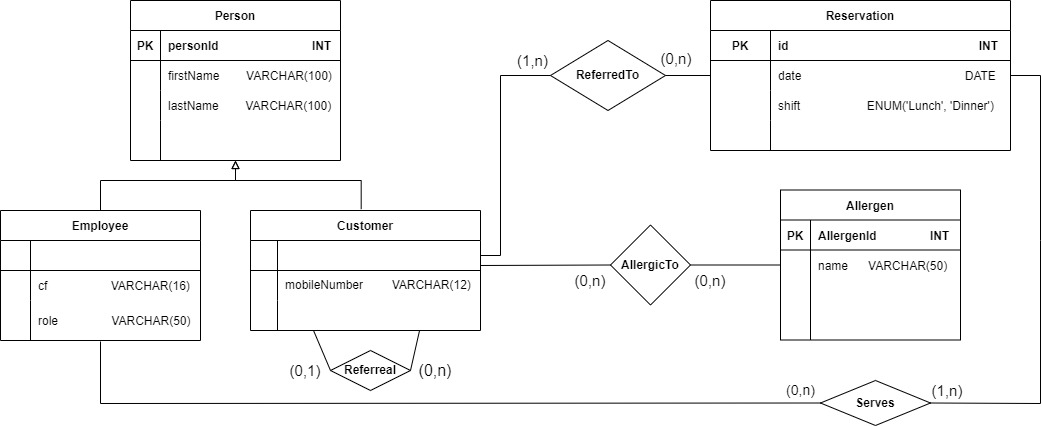
\includegraphics[width=\textwidth]{ER}
    \caption{ER Model}
    \label{fig:ermodel}
\end{figure}


\end{document}
